\section{Dynamic representation}

Let's consider the constant process $v(t,s)=v(s)$. 
In this scenario, once we determine the value of the experiment $v(s)$, we can derive the value of $v(t,s)$ for all time instants since its value remains unchanged.
This process is perfectly predictable.

In contrast, white noise is the opposite: it is a completely unpredictable process. 

Other processes lie between these two extremes.
Consequently, we can decompose a process into two parts: one purely deterministic and one purely non-deterministic:
\[v(t)=\tilde{v}(t)+\widehat{v}(t)\]
For $\tilde{v}(t)$, the knowledge of the past is sufficient to predict a value at a certain instant.
Note that $\tilde{v}(t)$ and $\widehat{v}(t)$ are independent: 
\[\mathbb{E}\left[ \tilde{v}(t_1)\widehat{v}(t_2) \right]=\mathbb{E}\left[ \tilde{v}(t_1)\right]\underbrace{\mathbb{E}\left[\widehat{v}(t_2) \right]}_0 =0\]
The correlation is given by:
\begin{align*}
    \tilde{\gamma}_v(\tau)  &=\mathbb{E}\left[v(t)v(t+\tau)\right] \\
                            &=\mathbb{E}\left[\left(\tilde{v}(t)+\widehat{v}(t)\right)\left(\tilde{v}(t+\tau)+\widehat{v}(t+\tau)\right)\right] \\
                            &=\mathbb{E}\left[\tilde{v}(t)+\tilde{v}(t+\tau)\right]\mathbb{E}\left[\widehat{v}(t)+\widehat{v}(t+\tau)\right] \\
                            &=\tilde{\gamma}_{\tilde{v}}(\tau)+\tilde{\gamma}_{\widehat{v}}(\tau)
\end{align*}

The purely nondeterministic component can be expressed as:
\[\widehat{v}(t)=\sum_{i=-\infty}^{t}W(t,1)\eta(i)=\sum_{i=-\infty}^{t}W(t-1)\eta(i)=\sum_{k=0}^\infty W(k)\eta(t-k)\]
Here, $\eta(\cdot) \sim WN(0,\lambda^2)$. 
This formula can be expanded as:
\begin{align*}
\widehat{v}(t)  &= W(0)\eta(t) + W(1)\eta(t-1) + W(2)\eta(t-2) + \dots \\
                &= W(0)\eta(t) + W(1)z^{-1}\eta(t) + W(2)z^{-2}\eta(t) + \dots \\
                &= \underbrace{\left(W(0) + W(1)z^{-1} + W(2)z^{-2} + \dots\right)}_{\text{transfer function }W(z)} \eta(t)  \\
\end{align*}
The stability of this function $W(z)$ implies the stationarity of the process $\widehat{v}(t)$.
\begin{figure}[H]
    \centering
    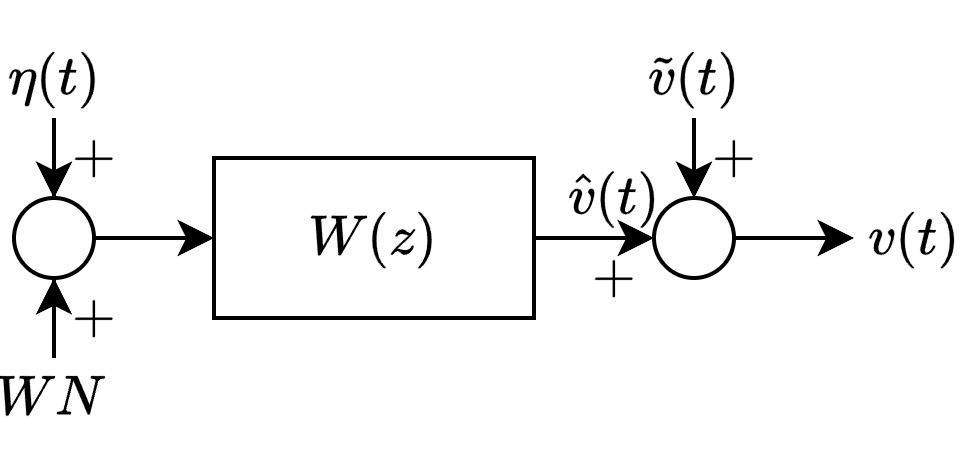
\includegraphics[width=0.4\linewidth]{images/dynamic.png} 
    \caption{Stochastic process composition}
\end{figure}

\subsection{Purely deterministic processes}
A purely deterministic process lacks any white noise component and can be expressed as:
\[\tilde{v}(t)=a_1\tilde{v}(t-1)+a_2\tilde{v}(t-2)+\dots+a_n\tilde{v}(t-n)\]
In operator notation, this becomes:
\begin{align*}
    \tilde{v}(t)    &= a_1z^{-1}\tilde{v}(t)+a_2z^{-2}\tilde{v}(t)+\dots+a_nz^{-n}\tilde{v}(t) \\
    \tilde{v}(t)    &= \underbrace{\left(a_1z^{-1}+a_2z^{-2}+\dots+a_nz^{-n}\right)}_{P(z)} \tilde{v}(t) \\
    0               &= P(z)\tilde{v}(t)
\end{align*}
This implies that $P(z)$ acts as a filter for $\tilde{v}(t)$. 
Consequently, we can predict all future values exactly.
The only restriction is that if such filtering is possible, then the function $\tilde{v}(t)$ has the following form:
\[\tilde{v}(t)=\alpha_1\lambda_1^t+\alpha_2\lambda_2^t+\dots+\alpha_n\lambda_n^t\]
Here, $\lambda_i$ are the zeros of $P(z)$, with $\left\lvert \lambda_i\right\rvert < 1$ for all $i$.
\begin{example}
    Consider a constant process $v(t)=v(t-1)$, which can be rewritten as $v(t)=\alpha 1^t$. 
    To extract the $P(z)$ function, we proceed as follows:
    \begin{align*}
        v(t)    &=z^{-1}v(t) \\
        0       &=v(t) - z^{-1}v(t) \\
        0       &=\left(1-z^{-1}\right)v(t)
    \end{align*}
    Hence, $P(z)=\left(1-z^{-1}\right)$. 
\end{example}
\begin{example}
    Consider a constant alternated process $v(t)=-v(t-1)$, which can be rewritten as $v(t)=\alpha (-1)^t$. 
    To extract the $P(z)$ function, we proceed as follows:
    \begin{align*}
        v(t)    &=-z^{-1}v(t) \\
        0       &=z^{-1}v(t) + v(t) \\
        0       &=\left(1+z^{-1}\right)v(t)
    \end{align*}
    Hence, $P(z)=\left(1+z^{-1}\right)$. 
\end{example}
\begin{example}
    Consider a constant sinusoidal process $v(t)=A \cos \left( \omega_0 t\right)$. 
    We can derive $P(z)$ as follows: 
    \begin{align*}
        P(z) &= \left(z-e^{j\omega_0}\right)\left(z-e^{-j\omega_0}\right) \\
             &= z^2+1-z\left(e^{j\omega_0}+e^{-j\omega_0}\right) \\
             &= z^2+1-2z\left(\dfrac{e^{j\omega_0}+e^{-j\omega_0}}{2}\right) \\
             &= z^2+1-2\cos (\omega_0)z
    \end{align*}
    To verify if $P(z)v(t)=0$, we perform a time shift of two:
    \begin{align*}
        P(z)v(t)&= \left(1-2\cos (\omega_0)z^{-2} z^{-2} \right)v(t) \\
                &= A \cos(\omega_0 t)-2\cos (\omega_0)A\cos(\omega_0(t-1))+A\cos(\omega_0(t-2)) \\
                &= A \cos(\omega_0 t)-2A \left[ \dfrac{1}{2}\cos\left( \omega_0t\right) +\cos\left(\omega_0(t-2)\right)  \right]+A\cos(\omega_0(t-2)) \\
                &= A \cos(\omega_0 t)-A\cos\left( \omega_0t\right) -A\cos\left(\omega_0(t-2)\right) +A\cos(\omega_0(t-2)) \\
                &= 0
    \end{align*}
    Thus, the process can also be written as a sum of exponential:
    \[v(t)=\alpha_1\lambda_1^t+\alpha_2\lambda_2^t\]
    Here, $\lambda_1$ and $\lambda_2$ needs to be replaced with the zeros of $P(z)$: 
    \[v(t)=\dfrac{A}{2}e^{j\omega_0t}+\dfrac{A}{2}e^{-j\omega_0t}\]
\end{example}